\documentclass{article}
\usepackage[utf8]{inputenc}
\usepackage{tikz}
\usepackage{pgf-umlcd}
\usepackage[margin=1.5cm]{geometry}

\usetikzlibrary{positioning, arrows.meta, calc, shapes.misc, matrix}

\title{Video Synchronization}
\author{Kevin Glocker}
\date{\today}

\begin{document}

\maketitle
% Remove page number
\pagenumbering{gobble} 

\begin{figure}[ht]
\begin{center}
\begin{tikzpicture}[
    scale=1,
    transform shape,
    line width=0.8pt,
    box/.style={draw, text centered, rounded corners, minimum height=2em, minimum width=8em}
]{
}
\end{tikzpicture}
\end{center}
\end{figure}

\begin{figure}[ht]
\begin{center}
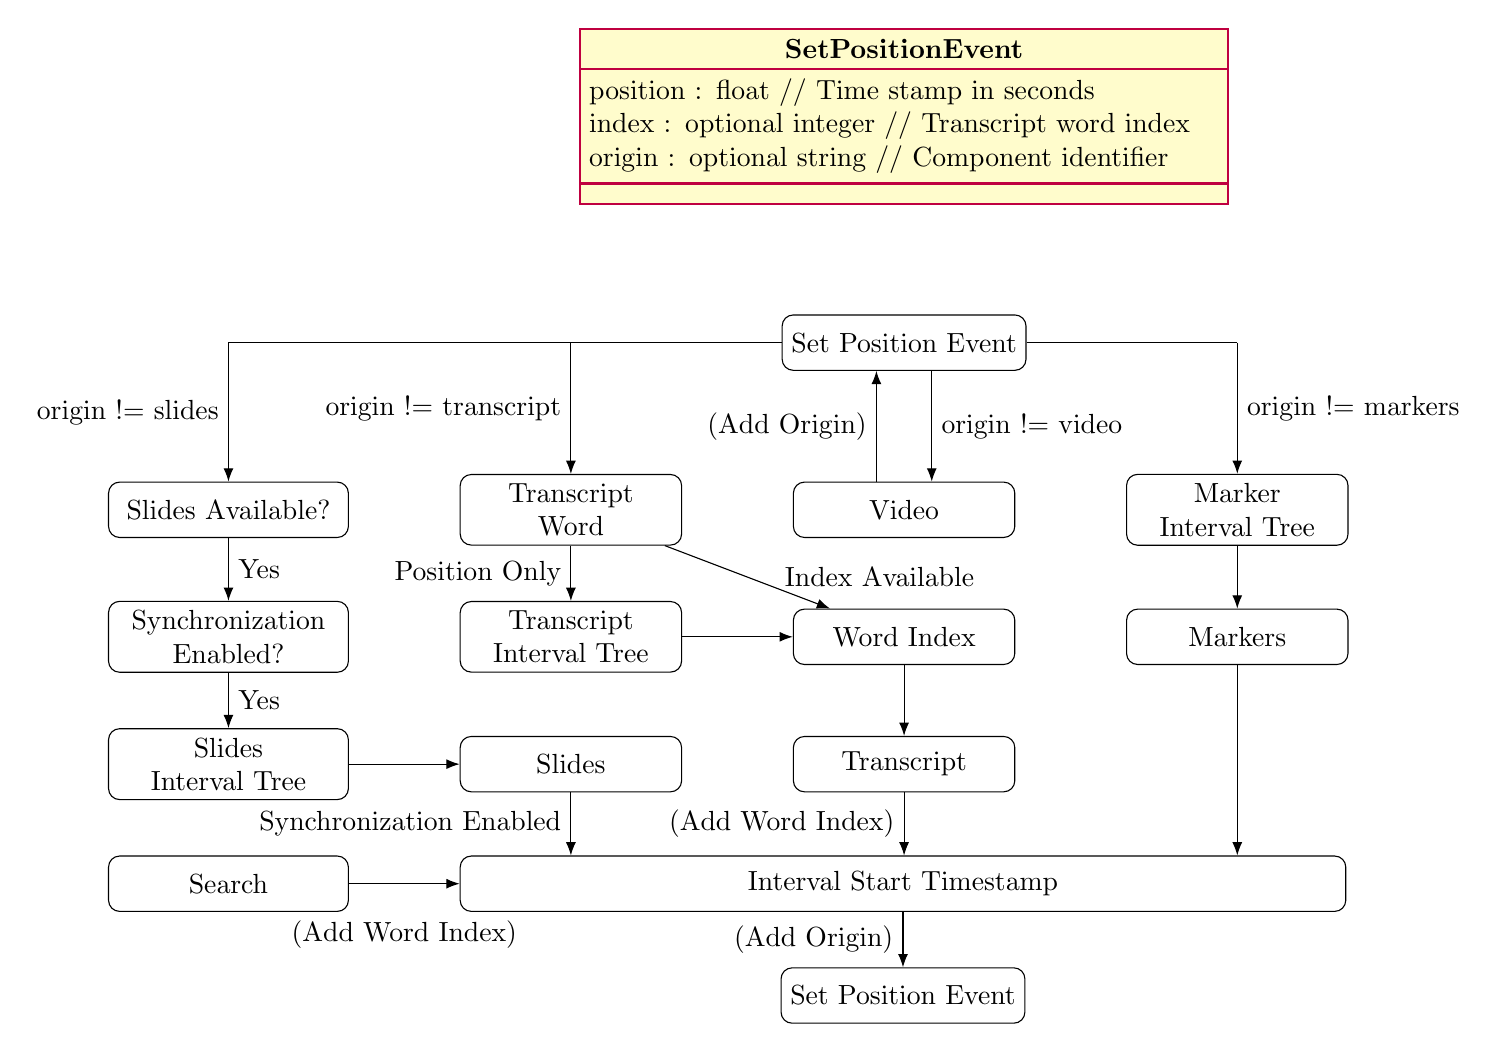
\begin{tikzpicture}[
    scale=1,
    transform shape,
    line width=0.8pt,
    box/.style={draw, text centered, rounded corners, minimum height=2em, minimum width=8em}
]{
    \begin{class}[text width=8cm]{SetPositionEvent}{0,0}
        \attribute{position : float // Time stamp in seconds}
        \attribute{index : optional integer // Transcript word index}
        \attribute{origin : optional string // Component identifier}
    \end{class}

    \node[box](position_event) at (0, -4){Set Position Event};
    \node[box, below=4em of position_event.south](video){Video};

    \node[box, right=4em of video.east, text width=6em](marker_tree){Marker\\Interval Tree};

    \node[box, left=4em of video.west, text width=6em](transcript_word){Transcript\\Word};

    \node[box, left=4em of transcript_word.west, text width=8em](slides_available){Slides Available?};

    % Transcript
    \node[box, below=2em of transcript_word.south, text width=6em](transcript_tree){Transcript\\Interval Tree};
    \node[box, right=4em of transcript_tree.east](word_index){Word Index};
    \node[box, left=4em of transcript_tree.west, text width=8em](slides_enabled_input){Synchronization\\Enabled?};
    \node[box, text width=8em, below=2em of slides_enabled_input.south](slides_tree){Slides\\Interval Tree};
    \node[box, right=4em of slides_tree.east](slides){Slides};

    \node[box, right=4em of word_index.east](markers){Markers};

    \node[box, right=4em of slides.east](transcript){Transcript};

    \node[box, below=2em of slides_tree.south, text width=8em](search){Search};
    \node[box, right=4em of search.east, minimum width=32em](interval_shared){Interval Start Timestamp};

    \node[box, below=2em of interval_shared.south](position_event_out){Set Position Event};

    \draw[-Latex]($(position_event.south) + (1em, 0)$) -- ($(video.north) + (1em, 0)$) node[midway, right]{origin != video};
    \draw[-Latex]($(video.north) - (1em, 0)$) -- ($(position_event.south) - (1em, 0)$) node[midway, left]{(Add Origin)};

    \draw(position_event) -- (marker_tree |- position_event);
    \draw[-Latex] (marker_tree |- position_event) -- (marker_tree) node[midway, right]{origin != markers};
    \draw(position_event) -- (slides_available |- position_event);
    \draw[-Latex](slides_available |- position_event) -- (slides_available) node[midway, left]{origin != slides};
    \draw[-Latex](transcript_word |- position_event) -- (transcript_word) node[midway, left]{origin != transcript};

    \draw[-Latex](marker_tree) -- (markers);

    \draw[-Latex](transcript_word) -- (transcript_tree) node[midway, left]{Position Only};
    \draw[-Latex](transcript_word) -- (word_index) node[midway, right, xshift=1em]{Index Available};
    \draw[-Latex](transcript_tree) -- (word_index);
    \draw[-Latex](word_index) -- (transcript);

    \draw[-Latex](slides_available) -- (slides_enabled_input) node[midway, right]{Yes};
    \draw[-Latex](slides_enabled_input) -- (slides_tree) node[midway, right]{Yes};
    \draw[-Latex](slides_tree) -- (slides);

    \draw[-Latex](search) -- (interval_shared) node[midway, below, yshift=-1em]{(Add Word Index)};
    \draw[-Latex](slides) -- (slides |- interval_shared.north) node[midway, left]{Synchronization Enabled};
    \draw[-Latex](transcript) -- (transcript |- interval_shared.north) node[midway, left]{(Add Word Index)};
    \draw[-Latex](markers) -- (markers |- interval_shared.north);

    \draw[-Latex](interval_shared) -- (position_event_out) node[midway, left]{(Add Origin)};
}
\end{tikzpicture}
\end{center}
\end{figure}

\vspace{2em}

\begin{itemize}
    \item Edge labels that aren't in parentheses mark conditions
    \item Where no edge exists for a condition, no action is performed
    \item Binary interval trees are used to map timestamps from the video to word indices, markers and slides
    \item When clicking on a word in the transcript or search results, selecting a marker or switching slides, the start timestamp of the word, marker or slide intervals are sent to the video
\end{itemize}

\end{document}
